\begin{singlespacing}
\chapter{The Standard Model and beyond}
\label{chapter:theory}
%
\begin{epigraphs}
\qitem{%
The idea that theorems follow from the postulates does not correspond to simple
observation.
If the Pythagorean theorem were found to not follow from the postulates, we
would again search for a way to alter the postulates until it was true.
Euclid's postulates came from the Pythagorean theorem, not the other way.}%
{Richard~Hamming,
\textit{The Unreasonable Effectiveness of Mathematics},
1980~\cite{hamming1980unreasonable}}
\end{epigraphs}
\end{singlespacing}
\noindent
The Standard Model encodes our best understanding of nature's fundamental
objects in their behaviours as particles.
From solid mathematical foundations, it accurately describes the physics
of particle interactions across a broad domain,
but that domain is bounded, so the Standard Model is not an ultimate theory of
everything.
Work continues to expand that boundary on both theoretical and experimental
fronts.
The current Standard Model is described in Section~\ref{sec:theory_sm},
along with its limitations and possible future directions.

Supersymmetry is an idea that has been applied to build plausible alternatives
to the Standard Model. and that may explain future experimental discoveries.
Since the main work of this thesis is a search for effects of supersymmetric
phenomena, Section~\ref{sec:theory_susy} discusses supersymmetry and
supersymmetric models.


\section{The Standard Model}
\label{sec:theory_sm}
The current Standard Model features fermions
(of four types in three generations),
which interact through forces mediated by vector bosons
and the scalar Higgs boson.
Massless gluons $g$ mediate the strong force,
the massless photon $\gamma$ mediates the electromagnetic force,
and very massive $W^+$, $W^-$, and $Z$ bosons mediate the weak force.
These fundamental particles of the Standard Model are summarized in
Table~\ref{tab:theory_particles_sm}.
The masses and charges of these particles are further detailed in
Table~\ref{tab:theory_particles_sm_properties}.

As a gauge field theory, the Standard Model has the symmetry group
$SU\!(3)_C \times SU\!(2)_L \times U\!(1)_Y$,
meaning that its Lagrangian is invariant under local operations of that group
on its fields in certain representations.
The subscript $_C$ refers to colour, $_L$ refers to left-chiral fields, and
$_Y$ refers to the weak hypercharge.

Gluons correspond to the eight generators of $SU\!(3)_C$, whose
subscript $_C$ indicates that they operate on colour-charge triplets of quarks.

Electromagnetic and weak forces are unified into the electroweak
interactions with four bosons $W^1$, $W^2$, $W^3$, and $B$ from the
$SU\!(2)_L$ and $U\!(1)_Y$ symmetries, respectively.
These would be massless if the symmetry were respected, but it is
`spontaneously' broken with the Higgs mechanism
\footnote{%
Historical accuracy prefers the name `Brout–Englert–Higgs mechanism', but
Peter~Higgs has reportedly suggested ``ABEGHHKtH mechanism'' to fully credit
contributing work~\cite{close2011infinity}.%
}~\cite{
higgs1964broken,
englert1964broken
},
which adds a complex doublet (equivalently four scalar fields) with an
associated potential to the model.
Minima of the potential lie in a gauge-symmetric set, and the choice made by
settling into one particular ground state spontaneously breaks the symmetry.
Around that chosen ground state, linear combinations of the electroweak fields
acquire masses while ``eating up''~\cite{rubakov1999classical} three of the
four scalar fields to yield the three massive weak bosons and the photon:
$W^1$ and $W^2$ mix into $W^+$ and $W^-$, while $W^3$ and $B$ mix into $Z$ and
$\gamma$.
The fourth scalar is the Higgs boson $h$~\cite{
glashow1959renorm,
weinberg1967model,
salam1959weak,
rubakov1999classical,
cottingham2007greenwood
}.

Fermion masses arise through their Yukawa interactions with the Higgs field.
The subscript $_L$ on $SU\!(2)_L$ indicates that the weak interaction only
couples to fermions in left-chiral doublets: $(\nu_e, e)_L$,
$(u, d)_L$ and their repeats across the three generations.
In each generational trio (such as $u$, $c$, $t$), all three fermions share the
same quantum numbers, but have different masses.
A second generational difference occurs in quarks and neutrinos through the
difference between their weak flavour eigenstates and the mass eigenstates of
their free propagation;
flavour and mass eigenstates are linearly related through unitary matrices:
the CKM matrix for the quarks~\cite{
cabibbo1963unitary,
kabayasji1973cpv
}
and the PMNS matrix for the neutrinos~\cite{
maki1962remarks,
thomson2013modern
}.

% using https://www.tablesgenerator.com/latex_tables
\begin{table}[tp]
\centering
\begin{tabular}{rrc}
\multirow{4}{*}{fermions} & \multirow{2}{*}{quarks}      & \makebox[5em]{\hfill $u$ \hfill $c$ \hfill $t$ \hfill}                    \\
                          &                              & \makebox[5em]{\hfill $d$ \hfill $s$ \hfill $b$ \hfill}                    \\[1ex]
                          & \multirow{2}{*}{leptions}    & \makebox[5em]{\hfill $e$ \hfill $\mu$ \hfill $\tau$ \hfill}               \\
                          &                              & \makebox[5em]{\hfill $\nu_e$ \hfill $\nu_\mu$ \hfill $\nu_\tau$ \hfill} \\[3ex]
\multirow{2}{*}{bosons}   & strong                       & \makebox[7em]{\hfill $g$ \hfill}                                          \\[1ex]
                          & electroweak & \makebox[7em]{\hfill $W^\pm\!\!$ \hfill $Z$\hfill $\gamma$ \hfill $h$ \hfill} \\
\end{tabular}
\caption[Particles of the Standard Model]{%
Particles of the Standard Model.
All fermions are spin-$1/2$, and all bosons are spin-$1$ except for the
spin-$0$ scalar Higgs boson $h$.
Fermions come in left- and right-chiralities, although the existence of
right-chiral neutrinos is not strictly confirmed.
See Table~\ref{tab:theory_particles_sm_properties} for details of their
properties.%
}
\label{tab:theory_particles_sm}
\end{table}

Early versions of the Standard Model had only two fermion generations and
no neutrino masses~\cite{
wells2020discovery,
bjorken1985november
},
but the third generation and non-zero neutrino masses are now observed;
for example, the third generation is shown by charge-parity ($\mathrm{CP}$
asymmetry in kaons~\cite{
cronin1964evidence,
kabayasji1973cpv
},
precise measurements of the $Z$ boson~\cite{
lep2006precision
},
and direct observations~\cite{
perl1977evidence,
herb1977observation,
abachi1995observation
};
neutrino masses are also necessary to explain their observed flavour
oscillations~\cite{
kamiokande1998measurement,
superk1998evidence,
superk1999measurement,
lsnd1998evidence
}.

Various theories can describe neutrino masses in the Standard Model, and it is
currently uncertain which form best describes nature;
this is both a limitation of the current Standard Model and an
opportunity for future refinement.
With future results, the Standard Model will continue to improve in its
correspondence with nature, and we discuss some such opportunities
for improvement in the next section.


% using https://www.tablesgenerator.com/latex_tables
\begin{table}[tp]
\centering
\begin{tabular}{ccccccc}
fermions                    & mass$\,\eV[G]$                      & $Q_{\mathrm{EM}}$    & $Y_L$                & $T^3_L$              & $Y_R$                & $T^3_R$              \\[0.2em]
leptons                     &                                     &                      &                      &                      &                      &                      \\[0.2em]
$e$                         & $5.11\times10^{-4}$                 & $-1$                 & $-\frac{1}{2}$       & $-\frac{1}{2}$       & $-1$                 & $0$                  \\
$\nu_e$                     & $\lesssim 1.1\times10^{-9}$         & $0$                  & $-\frac{1}{2}$       & $+\frac{1}{2}$       & $0$                  & $0$                  \\
$\mu$                       & $105.7$                             & $-1$                 & $-\frac{1}{2}$       & $-\frac{1}{2}$       & $-1$                 & $0$                  \\
$\nu_\mu$                   & $\lesssim 1.1\times10^{-9}$         & $0$                  & $-\frac{1}{2}$       & $+\frac{1}{2}$       & $0$                  & $0$                  \\
$\tau$                      & $1.777$                             & $-1$                 & $-\frac{1}{2}$       & $-\frac{1}{2}$       & $-1$                 & $0$                  \\
$\nu_\mu$                   & $\lesssim 1.1\times10^{-9}$         & $0$                  & $-\frac{1}{2}$       & $+\frac{1}{2}$       & $0$                  & $0$                  \\[1em]
quarks                      &                                     &                      &                      &                      &                      &                      \\[0.2em]
$u$                         & $2.16^{+0.49}_{-0.26}\times10^{-3}$ & $+\frac{2}{3}$       & $+\frac{1}{6}$       & $+\frac{1}{2}$       & $+\frac{2}{3}$       & $0$                  \\
$d$                         & $4.67^{+0.48}_{-0.17}\times10^{-3}$ & $-\frac{1}{3}$       & $+\frac{1}{6}$       & $-\frac{1}{2}$       & $-\frac{1}{3}$       & $0$                  \\
$c$                         & $1.27 \pm 0.02$                     & $+\frac{2}{3}$       & $+\frac{1}{6}$       & $+\frac{1}{2}$       & $+\frac{2}{3}$       & $0$                  \\
$s$                         & $93.4^{+8.6}_{-3.4}\times10^{-3}$   & $-\frac{1}{3}$       & $+\frac{1}{6}$       & $-\frac{1}{2}$       & $-\frac{1}{3}$       & $0$                  \\
$t$                         & $172.69\pm0.30$                     & $+\frac{2}{3}$       & $+\frac{1}{6}$       & $+\frac{1}{2}$       & $+\frac{2}{3}$       & $0$                  \\
$b$                         & $4.18^{+0.03}_{-0.02}$              & $-\frac{1}{3}$       & $+\frac{1}{6}$       & $-\frac{1}{2}$       & $-\frac{1}{3}$       & $0$                  \\[1em]
bosons                      & mass$\,\eV[G]$                      & $Q_{\mathrm{EM}}$    & $Y$                  & $T^3$                &                      &                      \\[0.2em]
$g$                         & $0$                                 & $0$                  & $0$                  & $0$                  &                      &                      \\
$W^+$                       & $80.4$                              & $+1$                 & $0$                  & $+1$                 &                      &                      \\
$W^-$                       & $80.4$                              & $-1$                 & $0$                  & $-1$                 &                      &                      \\
$Z$                         & $91.2$                              & $0$                  & $0$                  & $0$                  &                      &                      \\
$\gamma$                    & $0$                                 & $0$                  & $0$                  & $0$                  &                      &                      \\
$h$                         & $125.3 \pm 0.2$                     & $0$                  & $+\frac{1}{2}$       & $-\frac{1}{2}$       &                      &
\end{tabular}
\caption[Properties of Standard Model particles]{%
Properties of Standard Model particles~\cite{thomson2013modern,pdg2022ynf}.
% masses
Masses are given as determined in a recent review by the
Particle Data Group~\cite{pdg2022ynf}, which one should refer to for more
precision and more uncertainty estimates.
Uncertainty estimates are included only where they are relatively large.
% quark mass schemes
Quark masses are reported in the $\overline{\mathrm{MS}}$ scheme~\cite{
pdg2022ynf,
PhysRevD.18.3998
}.
% electric charge
The electric charge is given by $Q_{\mathrm{EM}} = Y + T^3$; one can check
that the left (L) and right (R) -handed fermions have equal electric charges
corresponding to their left and right weak hypercharges ($Y_L$ and $Y_R$)
and third weak isospin components ($T^3_L$ and $T^3_R$).
}
\label{tab:theory_particles_sm_properties}
\end{table}

\subsection{Lagrangian formulation}
\label{sec:theory_sm_lagrangian}
This section briefly reviews the Lagrangian of the Standard Model.
It is convenient to express such complicated mathematical expressions as sums
(and (possibly nested) sums)
of separate, labelled parts.
We employ this strategy.

The Standard Model Lagrangian (density) can be decomposed into this sum of
(partial Lagrangian) terms:
\begin{equation}
\label{eqn:theory_sm_lagrangian_top_sum}
\mathcal{L}_\mathrm{SM} =
\mathcal{L}_\mathrm{YM}
+ \mathcal{L}_\mathrm{WD}
+ \mathcal{L}_\mathrm{Yukawa}
+ \mathcal{L}_\mathrm{Higgs}
,
\end{equation}
which we define below;
$\mathcal{L}_\mathrm{YM}$ corresponds to the gauge bosons,
$\mathcal{L}_\mathrm{WD}$ corresponds to the fermions and their gauge
interactions,
$\mathcal{L}_\mathrm{Yukawa}$ corresponds to the Yukawa interactions between the
fermions and the Higgs,
and
$\mathcal{L}_\mathrm{Higgs}$ corresponds to the Higgs boson and its
potential~\cite{ramond1999journeys,pdg2022ynf}.
Note that this is only a condensed form of the full Standard Model Lagrangian,
which neglects much of its complexity.

\paragraph{Yang-Mills.}
The Yang-Mills summand $\mathcal{L}_\mathrm{YM}$ implements the gauge groups
$SU\!(3)_C$ (colour), $SU\!(2)_L$ (weak isospin), and $U\!(1)_Y$ (hypercharge),
each with a nested term respectively:
\begin{equation}
\label{eqn:theory_sm_lagrangian_top_ym}
\mathcal{L}_\mathrm{YM} =
\mathcal{L}_\mathrm{QCD}
+ \mathcal{L}_\mathrm{I_W}
+ \mathcal{L}_\mathrm{Y}
.
\end{equation}
All three Yang-Mills terms take similar forms:
\begin{align}
\label{eqn:theory_sm_lagrangian_top_ym_terms}
\mathcal{L}_\mathrm{QCD} &=
-\frac{1}{4g^2_3}
\sum_{A=1}^8 G^A_{\mu\nu} G^{\mu\nu A}
,\\
\mathcal{L}_\mathrm{I_W} &=
-\frac{1}{4g^2_2}
\sum_{a=1}^3 A^a_{\mu\nu} F^{\mu\nu a}
,\textrm{ and}\\
\mathcal{L}_\mathrm{Y} &=
-\frac{1}{4g^2_1} B_{\mu\nu} B^{\mu\nu}
.
\end{align}
Here, $g_3$, $g_2$, and $g_3$ are dimensionless constants.
They relate to colour, weak isospin, and hypercharge, respectively.
Furthermore, for colour,
\begin{equation}
G^A_{\mu\nu} =
\partial_\mu A^A_\nu - \partial_\nu A^A_\mu - f^{ABC} A^B_\mu A^C_\nu
,
\end{equation}
with $A, B, C \in \{1, 2, ..., 8\}$ indexing the eight gluon fields $A^B_\mu$ and
the $SU\!(3)_C$ structure function $f^{ABC}$.
For weak isospin,
\begin{equation}
F^a_{\mu\nu} =
\partial_\mu W^a_\nu - \partial_\nu W^a_\mu - \epsilon^{abc} W^b_\mu W^c_\nu
,
\end{equation}
with $a, b, c \in \{1, 2, 3\}$ indexing the vector bosons $W^a_\mu$ and
the $SU\!(2)_L$ structure function $\epsilon^{abc}$.
For hypercharge with the vector boson $B$,
\begin{equation}
B_{\mu\nu} =
\partial_\mu B_\nu - \partial_\nu B_\mu
.
\end{equation}

\paragraph{Weyl-Dirac.}
The Weyl-Dirac summand $\mathcal{L}_\mathrm{WD}$ implements the fermions and
their gauge interactions, and can be written:
\begin{equation}
\begin{split}
\mathcal{L}_\mathrm{WD} =
\sum_i^3
\Bigl(
& L^\dagger_i \sigma^\mu \mathcal{D}_\mu L_i
+ \bar e^\dagger_i \sigma^\mu \mathcal{D}_\mu \bar e_i \\
& + \mathbf{Q}^\dagger_i \sigma^\mu \mathcal{D}_\mu \mathbf{Q}_i
+ \mathbf{\bar u}^\dagger_i \sigma^\mu \mathcal{D}_\mu \mathbf{\bar u}_i
+ \mathbf{\bar d}^\dagger_i \sigma^\mu \mathcal{D}_\mu \mathbf{\bar d}_i
\Bigr)
,
\end{split}
\end{equation}
where each of the the $\mathcal{D}_\mu$ operators expresses a unique covariant
derivative that corresponds to the operand field.
These fermion fields are labelled
$L_i$ for lepton doublets,
$\bar e_i$ for lepton singlets,
$\mathbf{Q}_i$ for quark doublets,
and $\mathbf{\bar u}_i$ and $\mathbf{\bar d}_i$ for up- and down-type quark
singlets, respectively.
The notation $\bar x$ indicates the Dirac adjoint of $x$.
The three fermion generations are indexed by $i$.
The quark fields are in colour triplets.

\paragraph{Yukawa.}
The Yukawa term implements masses for the charged leptons by coupling
them to the scalar Higgs field $H$:
\begin{equation}
\mathcal{L}_\mathrm{Yukawa} =
i\hat L_i \bar e_j H^* Y^{[e]}_{ij}
+ i\mathbf{\widehat Q}_i \mathbf{\bar d}_j H^* Y^{[d]}_{ij}
+ i\mathbf{\widehat Q}_i \mathbf{\bar u}_j \tau_2 H Y^{[u]}_{ij}
+ [\textrm{c.c.}]
,
\end{equation}
in which $\tau_2$ contains weak isospin indices,
and $Y^{[e]}_{ij}$, $Y^{[d]}_{ij}$, $Y^{[u]}_{ij}$ are Yukawa coupling matrices
with shape $3\times3$ for the three fermion generations.
The notation $H^*$ indicates the complex conjugate of the complex scalar
Higgs field, and `c.c.' implies the complex conjugate of the expression to
its left.

\paragraph{Higgs.}
Finally, the Higgs term,
\begin{equation}
\mathcal{L}_\mathrm{Higgs} =
(\mathcal{D}_\mu H)^\dagger (\mathcal{D}^\mu H)
- \left[ -\mu^2 H^\dagger H + \lambda (H^\dagger H)^2 \right]
,
\end{equation}
contains the dynamics and potential for the scalar Higgs doublet.
The symbol $\mathcal{D}_\mu$ is a gauge-covariant derivative operator
specific to the Higgs field.
The notation $x^\dagger$ indicates the hermitian conjugate of $x$.
The potential terms are isolated into square brackets to highlight the negative
sign on the mass term $\mu^2$, which with the quartic term contributes to
spontaneous symmetry breaking~\cite{rubakov1999classical}.


\section{Opportunities for future Standard Models}
The Standard Model works very well within its domain.
This discussion therefore looks towards where an altered Standard Model could
improve its current abilities or to expand its generality to describe more of
the universe.

When `nobody knows' the answer to a riddle, the status lies somewhere between
two extremes:
either many answers are satisfactory with no clear best,
or no satisfactory answers are yet known.
We distinguish these two cases with the labels
\emph{uncertain} and \emph{unknown}, respectively:
the top quark mass is slightly \emph{uncertain},%
\footnote{%
The latest meta-analysis by the Particle Data Group estimates
$m(t) = 172.69 \pm 0.30\,\eV[G]$~\cite{pdg2022ynf}, as listed in
Table~\ref{tab:theory_particles_sm_properties}.
}
but the reconciliation of quantum field theory with general relativity is
mostly \emph{unknown}.

One real problem with the Standard Model is that algorithms to compute its
general consequences are unknown, since practical perturbative and discrete
lattice methods are limited.
Imprecise modelling weakens experimental results (anomalous or not),
but does not present an opportunity because it is common to the quantum field
theory that is used by all known viable models.
This section briefly reviews some other directions of positive change for
future models.


\subsection{Neutrino masses}
Neutrinos could be Dirac fermions with Yukawa masses and boring right-chiral
fields.
They could also have Majorana mass terms, for which the seesaw mechanism can
simultaneously generate the observed light neutrinos with very heavy `sterile'
neutrinos.
Or their masses could come from other operators without  introducing the
right-chiral fields~\cite{
thomson2013modern,
chala2021neutrino,
wells2020discovery
}.

The answer is uncertain, and new results from theory or experiment could
improve the Standard Model in the neutrino sector
by pinpointing a uniquely correct model.


\subsection{Gravitation and cosmology}
Gravity does not feature in the Standard Model, nor does it measurably impact
the particles in our experimental data.
Although gravitation is in another domain, the particle content of the
Standard Model does impact cosmology.

The universe contains dark matter which interacts with gravity but not much
with other forces; it is observed through galactic rotation curves,
gravitational lensing, and cosmic microwave background data,
but its composition is uncertain~\cite{
begeman1991rotation,
garrett2010dark,
planck2020results
}.
Dark matter candidates include new particles such as
sterile neutrinos~\cite{boyarsky2019sterile},
weakly interacting massive particles (WIMPs)~\cite{jungman1996wimp},
or
axion-like particles~\cite{kim2008axions},
but also macroscopic objects such as
primordial black holes~\cite{bernard2019primordial}.
Dark matter may well comprise a mixture of different components, and it would
be a success for future particle physics theories to pinpoint necessary dark
matter particles.

Other mysteries of cosmology include:
the small positive cosmological constant,
the inflation of the early universe,
and baryogenesis~\cite{
wells2020discovery,
riess1998observational
}.
Solutions to these mysteries all lie somewhere between uncertain and unknown,
but may not be entirely out of reach for future Standard Models.
For example, the Higgs field could plausibly have driven
inflation~\cite{bezrukov2008higgs},
and the Standard Model does slightly violate $\mathrm{C}$ and $\mathrm{CP}$,
both of which must be broken for baryogenesis~\cite{sakharov1991re}.


\subsection{Origins}
Why does the Standard Model have its structure?
Why is it configured with the observed values of our parameters?
Why do we even live in $3+1$ dimensional spacetime with quantum mechanics?
Answers to these questions are largely unknown, but would be
attractive features for a fundamental theory.

Certain Standard Model structures are quite general, and are parametrized such
that parts can be smoothly disabled if they do not describe nature.
For example, the strong interaction includes a parameter $\theta_\mathrm{CP}$
whose non-zero values would induce $\mathrm{CP}$ violation in the strong
sector.
Observations find that $\theta_\mathrm{CP}$ cannot be far from zero, and one
attractive feature of axion-like models is their requirement that
$\theta_\mathrm{CP} = 0$~\cite{
kim2008axions,
thomson2013modern,
martin2017particle
}.

Justified constraints on the model could have led to better predictions of
past data, and might extrapolate to new phenomena with their deeper
understanding of nature.
Attempts to relate the empirical parameters~\cite{
sato1979ratio,
beg1982gauge,
koide1983fermion,
denterria2012gaussian
}
or to derive the mathematical structures of physics~\cite{
goyal2010origin,
skilling2021abc,
axioms1010038
}
are curious, but will remain as curiosities only until they provide novel
benefits.


\subsection{Aesthetics}
In the search for improved models, heuristic criteria can help to identify
appealing candidates.
Two such criteria are `fine-tuning' and `naturalness', both of which are
aesthetic judgements about dimensionless model parameters.
Naturalness is opinion; only nature decides what is really natural,
but these criteria can still guide the scientific discourse towards useful
outcomes~\cite{wells2020discovery}.

Fine-tuning criteria dislike tight constraints, and naturalness contains
various ideas, of which one is that nice numbers should have moderate orders of
magnitude~\cite{giudice2008naturally}.
For example, $\theta_\mathrm{CP}$ is fine-tuned by the observational constraint
$\theta_\mathrm{CP} \lesssim 10^{-11}$, and the large $11$ in its exponent
defies naturalness.

Another example is the `hierarchy' problem of the Higgs boson mass $m(h)$,
which notes that new particles at a heavy mass scale $\Lambda$ induce changes
of $\Delta m(h)^2 = \mathcal{O}(\Lambda^2)$
through direct or indirect couplings.
With any new particles near the Planck scale $\Lambda \sim 10^{18}\,\eV[G]$,
implementing the observed $m(h) \sim 10^{2}\,\eV[G]$ therefore requires
finely-tuned cancellations between positive and negative contributions.
New fermions subtract from $m(h)$ and new scalars add by similar amounts,
so new models can implement this fine-tuning by inserting only matched sets of
fermions and bosons --- this is the strategy of supersymmetric models.


\section{Supersymmetric models}
\label{sec:theory_susy}
Supersymmetry is the concept of symmetry under the operation of exchanging
bosonic and fermionic states, and supersymmetric models use supersymmetry in
their construction.
Nature is not totally supersymmetric.
If it were, then there would be bosonic `superpartners' for each of the known
fermions (and vice versa) with the same masses and charges, and those
`sparticles' would have been seen long ago.
But supersymmetry might still participate in a broken condition if the
sparticles are hidden at larger masses.

Any new model must include the observational facts of the Standard Model,
and the Minimal Supersymmetric Standard Model (MSSM) satisfies this while
adding a school of new particles
who are registered in Table~\ref{tab:theory_particles_mssm}.

The MSSM matches each standard fermion to a pair of scalar
`sfermions' (left and right)
and each vector gauge field to a `gaugino' fermion
($\tilde g$, $\tilde W^1$, $\tilde W^2$, $\tilde W^3$, and $\tilde B$).
The Higgs field does not translate so directly, but is replaced with four
complex scalar fields
($H^+_u$, $H^0_u$ and $H^0_d$, $H^\pm_d$) with
gaugino superpartners
($\tilde H^+_u$, $\tilde H^0_u$ and $\tilde H^0_d$, $\tilde H^-_d$).
These fields mix into mass eigenstates whose compositions are uncertain:
the gaugino mixtures are the charged charginos $C^\pm_i$ and
neutral neutralinos $N_i$
(also labelled $\chargino_i$ and $\neutralino_i$~\cite{atlas2022searches}),
and each squark and slepton has two states that mix the left and right fields.
The four complex Higgs fields have eight degrees of freedom, of which three are
again eaten by the weak bosons to leave the reborn Standard Model Higgs boson $h$
and four new scalars~\cite{martin2016primer}.

% made using:
% https://www.tablesgenerator.com/latex_tables
\begin{table}[tp]
\centering
\begin{tabular}{rrc}
\multirow{5}{*}{bosons}   & Higgs                         & \makebox[7em]{\hfill ($h$) \hfill $H^0$ \hfill $A^0$ \hfill $H^\pm\!\!$ \hfill}             \\[1ex]
                          & \multirow{2}{*}{squarks}      & \makebox[5em]{\hfill $\tilde u$ \hfill $\tilde c$ \hfill $\tilde t$ \hfill}                  \\
                          &                               & \makebox[5em]{\hfill $\tilde d$ \hfill $\tilde s$ \hfill $\tilde b$ \hfill}                  \\[1ex]
                          & \multirow{2}{*}{sleptions}    & \makebox[5em]{\hfill $\tilde e$ \hfill $\tilde \mu$ \hfill $\tilde \tau$ \hfill}             \\
                          &                               & \makebox[5em]{\hfill $\tilde \nu_e$ \hfill $\tilde \nu_\mu$ \hfill $\tilde \nu_\tau$ \hfill} \\[3ex]
\multirow{3}{*}{fermions} & gluinos                       & \makebox[5em]{\hfill $\tilde g$ \hfill}                                        \\[1ex]
                          & \multirow{2}{*}{gauginos}     & \makebox[5em]{\hfill $\tilde C^\pm_1\!\!$ \hfill $\tilde C^\pm_2\!\!$ \hfill} \\
                          &                               & \makebox[7em]{\hfill $\tilde N_1\!$ \hfill $\tilde N_2\!$ \hfill$\tilde N_3\!$ \hfill$\tilde N_4\!$ \hfill} \\
\end{tabular}
\caption[%
Particles of the Minimal Supersymmetric Standard Model%
]{%
Particles of the Minimal Supersymmetric Standard Model
in their mass eigenstates~\cite{martin2016primer}, in addition to the
Standard Model particles of Table~\ref{tab:theory_particles_sm}.
The standard Higgs boson ($h$) is repeated here with its new pals.
Sparticles are marked with tildes $\tilde{~}$.
All listed bosons are spin-$0$ and all listed fermions are spin-$1/2$.
}
\label{tab:theory_particles_mssm}
\end{table}

Current observations do limit the masses and mixings of this new
school of MSSM particles, but their values remain very uncertain and in need
of new experimental constraints.
Diverse observable effects can be induced by parameter choices,
so we use simplified models to coarsely characterize interesting and plausible
examples.
Such simplified models feature only a few free variables, and decouple other
effects by, for example, sending masses to extremely large values or assuming
no mixing~\cite{
atlas2022searches,
alwall2009simplified,
alves20212simplified
}.
Experimental data only provide lower bounds on the masses of these new
particles, and those bounds depend strongly on the simplifying assumptions
made in each case. Some moderately-general bounds have been assigned however,
and examples of these bounds are listed in
Table~\ref{tab:theory_particles_mssm_mass_limits}.
Longer listings of limits in many special cases can be found in the
Particle Data Group review~\cite{pdg2022ynf}.


% made using:
% https://www.tablesgenerator.com/latex_tables
\begin{table}[tp]
\centering
\begin{tabular}{cc}
fermions                                        & mass limit$\,\eV[G]$ \\[0.2em]
$\neutralino_1$ (stable)                        & $> 46$         \\
$\neutralino_1$ (unstable)                      & $> 380$        \\
$\neutralino_2$, $\neutralino_3$, $\neutralino_4$ & $> 750$        \\
$\chargino_1$, $\chargino_2$                     & $> 94$         \\[1em]
bosons                                          & mass limit$\,\eV[G]$ \\[0.2em]
$\tilde \nu_e$, $\tilde \nu_\mu$, $\tilde \nu_\tau$ & $> 94$       \\
$\tilde e$                                      & $> 107$        \\
$\tilde \mu$                                    & $> 94$         \\
$\tilde \tau$                                   & $> 81.9$       \\
$\tilde u$, $\tilde d$, $\tilde c$, $\tilde s$     & $> 1220$       \\
$\tilde b$                                      & $> 1270$       \\
$\tilde t$                                      & $> 1310$       \\
$\tilde g$                                      & $> 2300$
\end{tabular}
\caption[%
Mass limits for particles of the Minimal Supersymmetric Standard Model%
]{%
Mass limits for particles of the Minimal Supersymmetric Standard Model as
reported under by the Particle Data Group under loose
assumptions, quoted at ``$\mathrm{CL}=95.0\%$''~\cite{pdg2022ynf}.
The charges of these particles equal the charges of their Standard Model
partners, which are listed in
Table~\ref{tab:theory_particles_sm_properties}.
\\[0.4em]
All of these limits assume R-parity conservation and various other,
instance-specific constraints.
For example, the limit of
$m(\neutralino_2,\neutralino_3,\neutralino_4) > 750\,\eV[G]$
assumes that $m(\neutralino_1) < 100\,\eV[G]$.
Many stronger constraints are reported within the constraints of simplified
models.
Limits on R-parity violating models differ, and can be either stronger or
weaker.
In the stable $\neutralino_1$ case, the $\neutralino_1$ is the lightest
supersymmetric particle and a dark matter candidate;
in the unstable $\neutralino_1$ case, it rapidly decays.
Stronger limits can be set for particles that live long enough to decay within
the sensitive materials of collider detectors.
\\[0.4em]
All listed bosons are spin-$0$ and all listed fermions are spin-$1/2$.
}
\label{tab:theory_particles_mssm_mass_limits}
\end{table}

Various mechanisms could spontaneously break supersymmetry.
Gravitational mechanisms exist, but one model considered in this thesis uses
Gauge-Mediated Supersymmetry Breaking (GMSB),
which adds yet more elusive fields:
a `secluded' sector which breaks the symmetry, and
a `messenger' sector which
communicates that breaking effect back to the observable sector.
Such models also add a spin-$3/2$ `gravitino' ($\gravitino$),
which should be light and whose helicity $\pm1/2$ components would interact
in collider physics~\cite{
giudice1999gmsb,
dine1982pheno,
martin2016primer
}.

All supersymmetric models considered in this thesis conserve $R$-parity
\begin{equation}
P_R = (-1)^{3(B - L) + 2s}
\end{equation}
(with baryon number $B$, lepton number $L$ and spin $s$)
in their interactions~\cite{
farrar1978rparity,
martin2016primer
}.
Conservation of $R$-parity usefully prevents proton decays,
but also makes the Lightest Supersymmetric Particle (LSP) a plausible
WIMP dark matter candidate since it cannot decay to purely Standard Model
particles.
Providing this LSP dark matter candidate through a production mechanism
that is accessible at the LHC is a strong motivating factor both for
supersymmetric models and for the experimental search of this thesis.

Supersymmetric modelling successfully predicted the lightest Higgs boson
mass to be $\lesssim 130\,\eV[G]$ long before its observation at
$125\,\eV[G]$~\cite{
espinosa1992higgs,
espinosa1993upper,
quiros1997constraints,
wells2020discovery,
atlas2012higgs,
atlas2012combined,
cms2012higgs
}.
This prediction, however, assumed a mass scale below $1\,\eV[T]$,
and observations at the LHC are now limiting sparticle masses into
super-$\eV[T]$ territory (in specific simplified models).
Such observational limits are also troublesome for the hierarchy problem,
because large superpartner masses introduce fine-tuning problems of their
own~\cite{martin2016primer}.
Despite its current lack of observational evidence,
supersymmetry remains a tool for building theoretically plausible
models, and might help us to understand future discoveries
that could be made with data from the \atlas\ detector.

\subsection{Lagrangian formulation}
\label{sec:theory_susy_lagrangian}
In Section~\ref{sec:theory_sm_lagrangian}, we presented a highly compressed
summary of the Standard Model Lagrangian.
Despite its minimality, the MSSM is a far more complicated theory than the
Standard Model, and the expression of its Lagrangian formulation is
far larger.
This section therefore presents and even more compressed summary of the
Lagrangian formulation of the MSSM.

Although any viable theory must include the Standard Model in an appropriate
appropriation, the Standard Model's Lagrangian need not be explicitly included.
Indeed, it is not convenient to express the MSSM's Lagrangian as an add-on to
the Standard Model. It stands alone.

A convenient first decomposition of the MSSM Lagrangian's parts splits it into
four parts:
\begin{equation}
\mathcal{L}_\mathrm{MSSM} =
\mathcal{L}_\mathrm{SUSY}
+ \mathcal{L}_\mathrm{soft}
+ \mathcal{L}_\mathrm{GF}
+ \mathcal{L}_\mathrm{ghost}
,
\end{equation}
in which
$\mathcal{L}_\mathrm{SUSY}$ is the supersymmetric part,
$\mathcal{L}_\mathrm{soft}$ is the a `softly' breaking part
(which is necessary because supersymmetry is not an unbroken symmetry of
nature),
and
$\mathcal{L}_\mathrm{GF}$ and $\mathcal{L}_\mathrm{ghost}$
are two additions that are necessary for quantization of the
theory~\cite{kuroda1999complete}.

\paragraph{Supersymmetry.}
The supersymmetric summand $\mathcal{L}_\mathrm{SUSY}$ contains numerous terms
that implement the main particle content of the MSSM.
These terms are not trivially expressed as Lagrangian densities in
four-dimensional spacetime, but are more fundamentally also integrated over
`superspace' coordinates~\cite{martin2016primer, kuroda1999complete}.
It contains kinetic terms for the gauge bosons, gauginos, fermions, sfermions,
Higgs, and higgsinos fields.
It also implements interactions between these fields,
including interactions between the fermions and gauge bosons,
Yukawa interactions between the fermions and Higgs fields and higgsinos,
and interactions between the gauge bosons and Higgs fields.
The gauge-Higgs interactions produce masses for the gauge bosons.
Other terms directly implement masses for mixtures of the higgsino fields.

\paragraph{Soft breaking.}
With no known mechanism for supersymmetry breaking,
the term $\mathcal{L}_\mathrm{soft}$ is expressed as a maximally general form
with $30$ free parameters, which have only weak constraints to ensure
symmetries in the theory.
It includes possible mass terms for the constituent fields, as well as scalar
interaction vertices.

\paragraph{Others.}
The gauge-fixing term $\mathcal{L}_\mathrm{GF}$ ensures that the gauge boson
propagators take the Standard Model form.
The ghost term $\mathcal{L}_\mathrm{ghost}$ introduces special scalar fields
that interact with bosons in the theory, but which have no effect at tree-level
but are necessary for self-consistency of the theory in loop
diagrams~\cite{martin2016primer, kuroda1999complete}.


\subsection{Specific simplified models}
Two specific simplified supersymmetric models are studied in this thesis.
These models were selected for the \atlas\ $\twoljets$
search~\cite{atlas2022searches},
presented in Chapter~\ref{chapter:2ljets},
because they are well-studied but not-yet excluded models that can affect the
data in its targetted signature of data with two charged leptons,
hadronic jets, and missing transverse momentum.
Within the context of $\twoljets$, we name these two simplified models
`C1N2' and `GMSB'.

Both of these simplified models are micro-examples of complete new theories
that offer solutions to the hierarchy
problem~\cite{Sakai:1981gr,SUSY-2018-02}.
Both models also conserve R-parity, so they satisfy constraints from proton
decay and introduce a stable, neutral dark matter candidate in their respective
LSPs~\cite{Ellis:1983ew}.
Many \atlas\ searches distribute their efforts across many simplified models;
this search embodies just one tile in the mosaic of \atlas's SUSY programme.

\paragraph{C1N2.}
`C1N2' is a restricted subset of the MSSM in which the only active SUSY
particles
are the lightest chargino ($\chargino_1$)
and the lightest two neutralinos ($\neutralino_1$, $\neutralino_2$).
The name `C1N2` is an abbreviation to
`Chargino 1' concatenated with `Neutralino 2'.
This model is active in the electroweak sector of the MSSM, which has received
increased interest in recent years because the LHC is more sensitive to models
in the strong sector.
Existing LHC results have have already ruled out many strongly-interacting
models up to multi-$\eV[T]$ mass scales, but some interesting phase space
remains in the electroweak sector.
We choose to study C1N2 to attend to this remaining phase space.

Chargino-neutralino pairs are produced in proton collisions via off-shell
$W$ boson propagators in this model.
The targeted experimental signature is achieved by decays of these gauginos
to the $\neutralino_1$ LSP via emission of Standard Model particles.

\paragraph{GMSB.}
As described earlier in Section~\ref{sec:theory_susy}, GMSB models offer a
general mechanism to break supersymmetry by communicating some symmetry
breaking down from high mass scales~\cite{Meade:2008wd,SUSY-2018-02}.
The specific GMSB model used in the \atlas\ $\twoljets$ search
(and referred to as simply GMSB in its context) is a simplified model that
captures broad patterns of plausible behaviours in an experimentally pragmatic
format.
Under this GMSB model, visible signatures are generated by decays higgsino-like
neutralinos to Standard Model particles and a gravitino LSP, specifically
$\neutralino_1 \to Z/h + \gravitino$ from each side of a
$\neutralino_1 \neutralino_1$ pair production event.

We are experimentally interested in this decay mode because the $Z$ and Higgs
bosons can decay to diverse Standard Model decay products.
Again, the \atlas\ $\twoljets$ search chooses to target this model because
a significant decay mode includes $Z \to \ell^+\ell^-$, jets, and invisible
particles giving missing transverse momentum.
This simplified GMSB model also chooses a
`compressed' mass spectrum, meaning small differences between the masses of
$\neutralino_1$ and the slightly-heavier $\chargino_1$ and $\neutralino_2$.
This choice creates diverse initial states, since the hard scatter events can
emit various different pairs of heavier gaugino species and they will all decay
via unobservably soft emissions to produce the same
$\neutralino_1 \neutralino_1$ target
pair~\cite{atlas2022searches,hepdata.116034}.


\subsubsection{Cross-sections}
A substantial production cross-section is a necessary condition for a process
to be observable with finite data.
The Run~2 dataset studied by our $\twoljets$ search comprises
$L = 139\,\mathrm{fb}^{-1}$
of proton-proton collisions, meaning that a process with production
cross-section $\sigma = 1\,\mathrm{fb}$
yields a Poisson mean of $\mu = L \sigma = 139$ events.
To achieve a mean of one event in the dataset,
below which it becomes exceedingly hard to observe,
a process needs a cross-section at least $1 / L \approx 7\,\mathrm{pb}$.

Cross-sections for the $\twoljets$ C1N2 and GMSB models are determined by two
factors: production cross-section and the decay branching fraction.
Each process pair-produces some heavy parent particles, so their production
cross-sections scale down with the parent particle mass
as both parton distribution hard-scatter matrix element
are pushed to harder scales.
For mass scale $q$, these three factors combine to an rapidly decaying scaling
of cross-section with parent mass, which goes very roughly like
$\sigma \sim q^{-6}$ in the several-hundred-$\,\eV[G]$ regime.
Example production cross-sections for similar models are displayed in
Figure~\ref{fig:theory_susy_xs}.
Branching fractions in decay further reduce the observable cross-sections in
our selected decay channels; however, these are constant factors that do not
scale with parent mass.

\begin{figure}[tp]
\centering
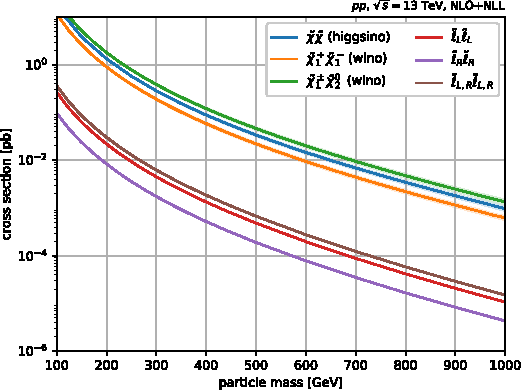
\includegraphics[width=0.9\textwidth]{figures/theory_pdg_susy_xsec.pdf}
\caption[
Cross-section scaling of some supersymmetric pair production modes
]{%
Cross-section scaling of some supersymmetric pair production modes
in models similar to the $\twoljets$ C1N2 and GMSB simplified models.
Note the similar scaling parent particle mass  for all gaugino and slepton
production modes shown;
this effect is due to fundamental properties of parton distribution functions
and scattering matrix-elements, and is not unique to supersymmetry.
These cross-sections do not include branching fraction factors, which are
needed to determine the C1N2 and GMSB cross-sections.
This figure is reproduced from~\cite{pdg2022ynf}.
\\[0.4em]
The label `wino` indicates that the gaugino mixtures mostly comprise the
superpartners of the $W$ fields, and `higgsino` indicates that they instead
comprise higgsino fields.
\\[0.4em]
Cross-sections below around $7\,\mathrm{pb}$ are expected to produce no
events in our $139\,\mathrm{fb}^{-1}$ of data.
}
\label{fig:theory_susy_xs}
\end{figure}


\TODO{example numbers}

% this comment activates enlarged spacing for the final paragraph lol
